
\documentclass[12pt]{exam}
\usepackage{amsthm}
\usepackage{libertine}
%\usepackage[utf8]{inputenc}
\usepackage[margin=1in]{geometry}
\usepackage{amsmath,amssymb}
\usepackage{multicol}
\usepackage[shortlabels]{enumitem}
\usepackage{siunitx}
\usepackage{cancel}
\usepackage{graphicx}
\graphicspath{{./}}
\usepackage{pgfplots}
\usepackage{hyperref}
\usepackage{listings}
\usepackage{tikz}
\usepackage{minted}
\def\code#1{\texttt{#1}}
\usepackage{amssymb}
\usepackage{xcolor}
% for plotting
\usepackage{pgfplots}
\pgfplotsset{compat=1.16}
\usepackage{tikz}
\usetikzlibrary{arrows.meta}

\newcommand{\quotebox}[1]
{
  \begin{center}
    \fcolorbox{white}{blue!15!gray!15}{
      \begin{minipage}{0.7\linewidth}\vspace{10pt}
        \center
        \begin{minipage}{0.8\linewidth}{\space\Huge``}{\setlength{\parindent}{1.5em}#1}{\hspace{1.5em}\break\null\Huge\hfill''}
        \end{minipage}
        \smallbreak
      \end{minipage}
    }
\end{center}
}

%\DeclareUnicodeCharacter{2212}{-}


\let\oldemptyset\emptyset
\let\emptyset\varnothing

\hypersetup{
    colorlinks=true,
    linkcolor=blue,
    filecolor=magenta,      
    urlcolor=cyan,
    pdftitle={Overleaf Example},
    pdfpagemode=FullScreen,
    }
    
\urlstyle{same}

\pgfplotsset{width=10cm,compat=1.9}
\usepgfplotslibrary{external}
\tikzexternalize

\newcommand{\class}{Math 415} % This is the name of the course 
\newcommand{\examnum}{Homework-6} % This is the name of the assignment
\newcommand{\examdate}{Oct 26} % This is the due date
\newcommand{\timelimit}{}

\newcommand{\BO}{\mathcal{O}}




\begin{document}
\pagestyle{plain}
\thispagestyle{empty}

\noindent
\begin{tabular*}{\textwidth}{l @{\extracolsep{\fill}} r @{\extracolsep{6pt}} l}
\textbf{\class} & \textbf{Name:} & \textit{Zhenzhao Tu}\\ %Your name here instead, obviously 
\textbf{\examnum} &&\\
\textbf{\examdate} &&\\
\end{tabular*}\\
\rule[2ex]{\textwidth}{2pt}
% --


\section*{Problem 1}
\begin{enumerate}
	\item \[ \dot{x} = x-y, \quad \dot{y} = 1-e^x \] 
	We can find the Jacobian matrix of the system:
	\[ J = \begin{bmatrix}
		1 & -1 \\
		-e^x & 0
	\end{bmatrix} \quad \text{at} \quad (0,0) \quad \text{is} \quad J(0,0) = \begin{bmatrix}
		1 & -1 \\
		-1 & 0
	\end{bmatrix} \]
	Then we can find the eigenvalues and eigenvectors of $J(0,0)$:
	\[ \lambda_1 = \frac{1+\sqrt{5}}{2}, \quad \lambda_2 = \frac{1-\sqrt{5}}{2} \quad \text{and} \quad v_1 = \begin{bmatrix}
		\frac{-1-\sqrt{5}}{2} \\
		1
	\end{bmatrix}, \quad v_2 = \begin{bmatrix}
		\frac{-1+\sqrt{5}}{2} \\
		1
	\end{bmatrix} \]
	Then we can use nullclines to find the phase portrait of the system:
	\begin{figure}[H]
		\centering
		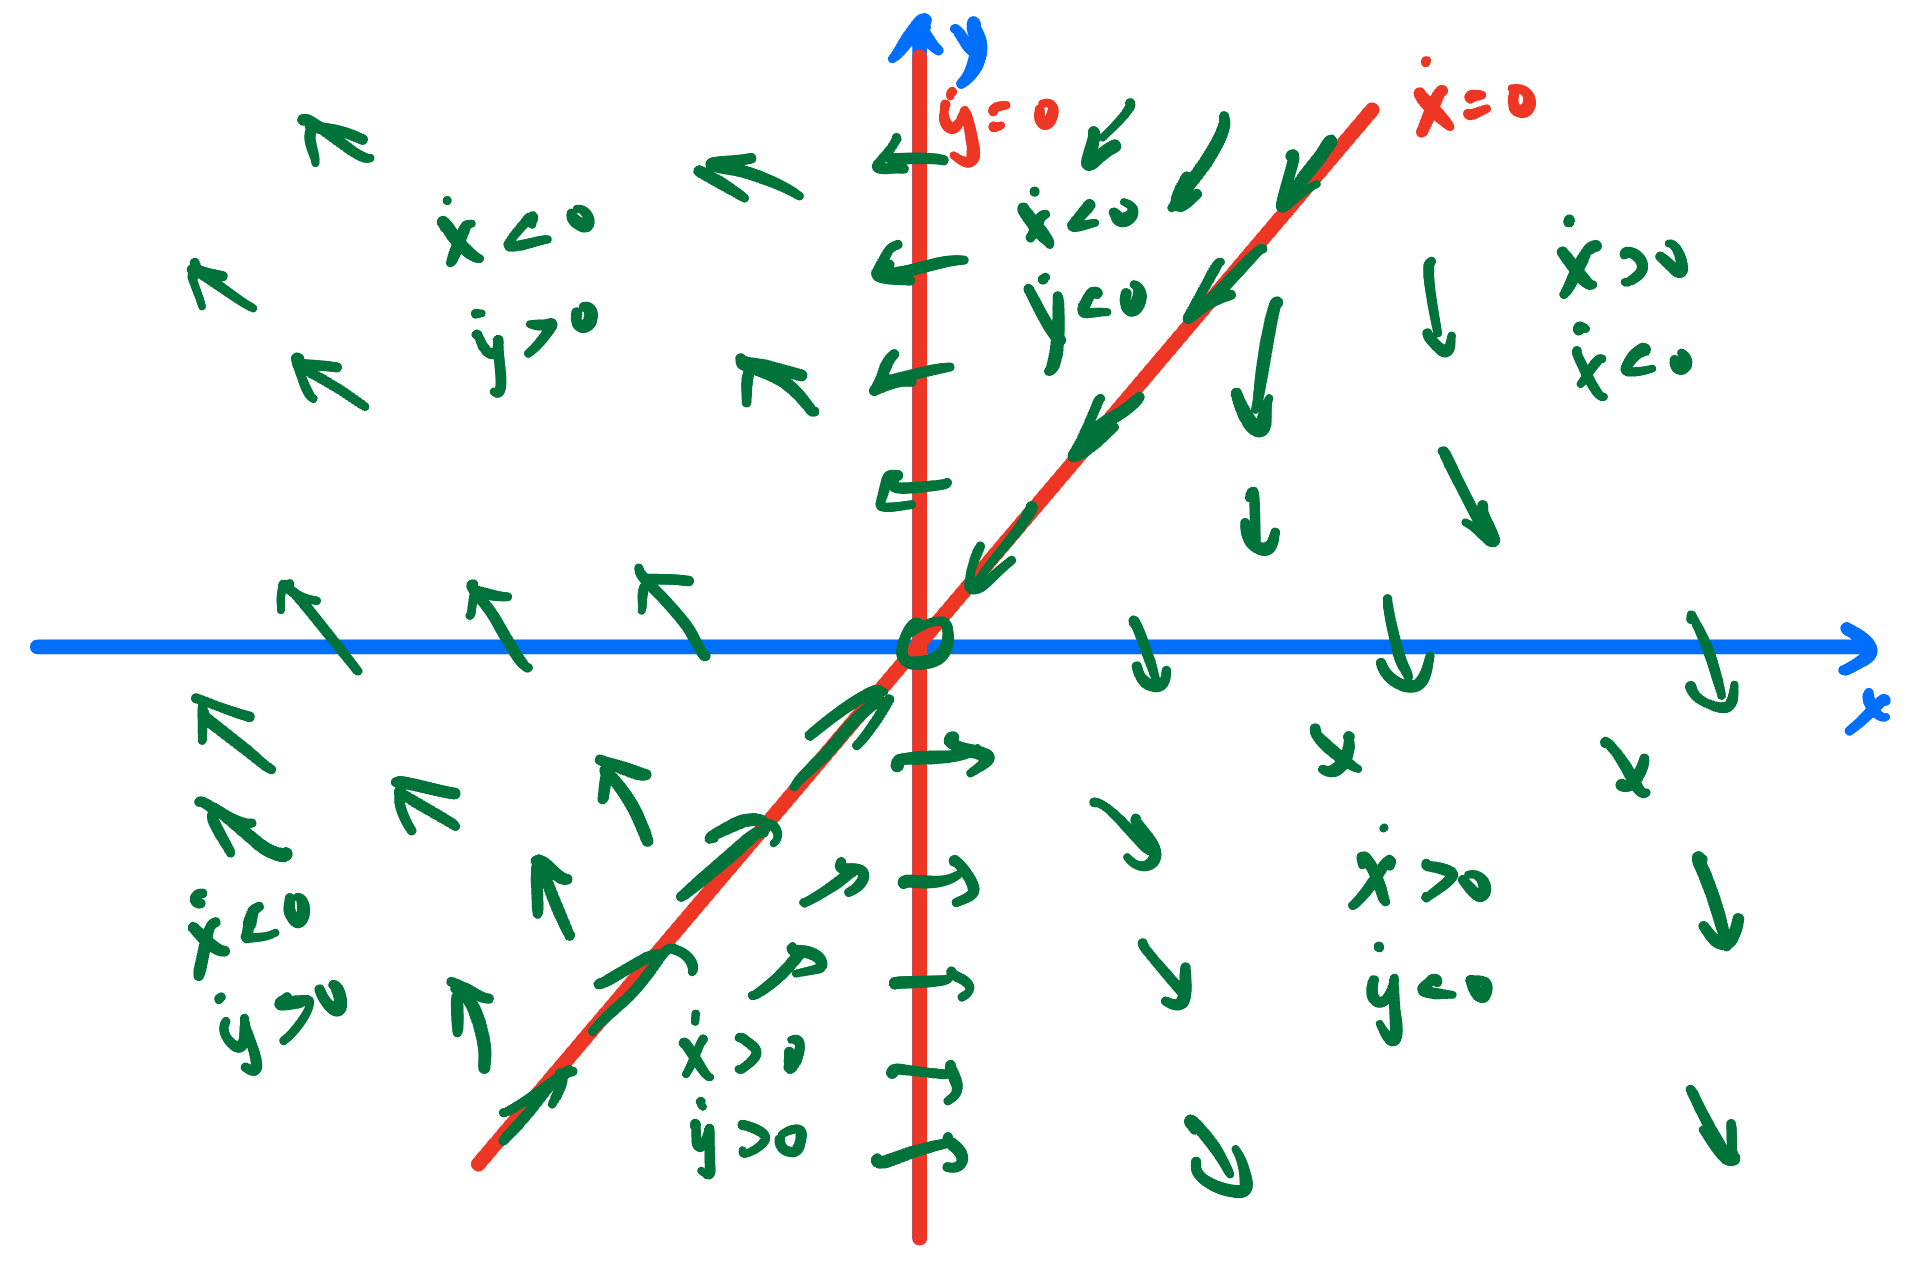
\includegraphics[width=0.9\linewidth]{1a.jpeg}
		\caption{Phase portrait of the system}
		\label{fig:1a}
	\end{figure}

	\newpage
	\item \[ \dot{x} = y, \quad \dot{y} = x(y+1)-1 \]
	We can find the Jacobian matrix of the system:
	\[ J = \begin{bmatrix}
		0 & 1 \\
		y+1 & x
	\end{bmatrix} \quad \text{at} \quad (1,0) \quad \text{is} \quad J(1,0) = \begin{bmatrix}
		0 & 1 \\
		1 & 1
	\end{bmatrix} \]
	Then we can find the eigenvalues and eigenvectors of $J(1,0)$:
	\[ \lambda_1 = \frac{1+\sqrt{5}}{2}, \quad \lambda_2 = \frac{1-\sqrt{5}}{2} \quad \text{and} \quad v_1 = \begin{bmatrix}
		\frac{-1+\sqrt{5}}{2} \\
		1
	\end{bmatrix}, \quad v_2 = \begin{bmatrix}
		\frac{-1-\sqrt{5}}{2} \\
		1
	\end{bmatrix} \]
	Then we can use nullclines to find the phase portrait of the system:
	\begin{figure}[H]
		\centering
		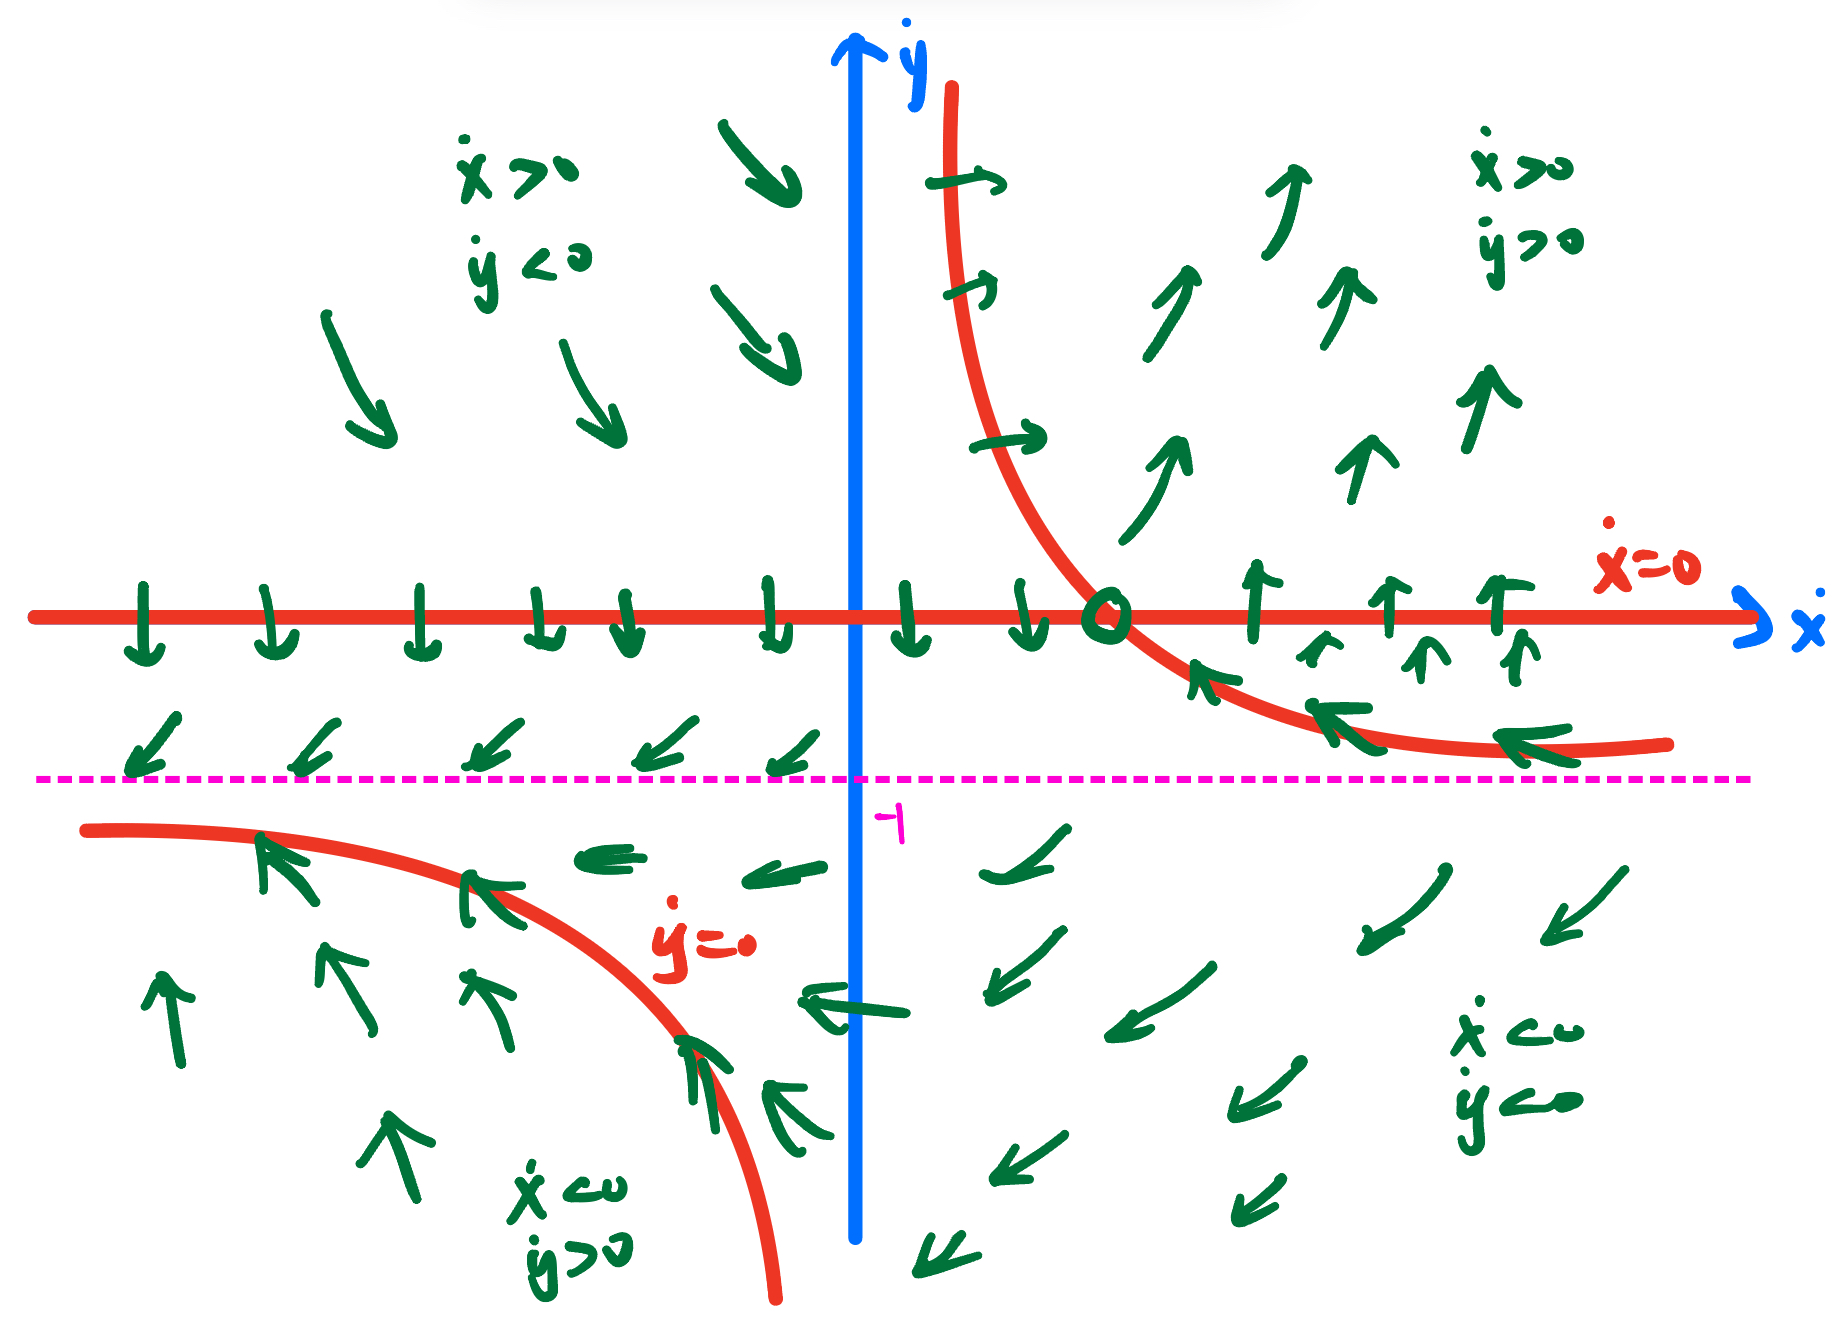
\includegraphics[width=0.9\linewidth]{1b.jpeg}
		\caption{Phase portrait of the system}
		\label{fig:1b}
	\end{figure}
\end{enumerate}

\section*{Problem 2}
Let $D$ be the open disk $x^2+y^2<4$. Consider the system
\[ \dot{x} = y, \quad \dot{y} = -x + (1-x^2-y^2)y \]
\begin{enumerate}[(a)]
	\item To satisfy the existence and uniqueness theorem, we need to show that $f(x,y)$ is continuous and all partial derivatives of $f(x,y)$ are continuous for all $(x,y) \in D$.
	\begin{proof}
		\textbf{f is continuous:} $\dot{x} = y$ is continuous in $D$ since it is linear function. $\dot{y} = -x + (1-x^2-y^2)y$ is continuous in $D$ since it is a polynomial function. Therefore, $f(x,y)$ is continuous in $D$. \\
		\textbf{Partial derivatives of f are continuous:} For $\dot{x}$ we have $\frac{\partial f}{\partial x} = 0$ and $\frac{\partial f}{\partial y} = 1$. For $\dot{y}$ we have $\frac{\partial f}{\partial x} = -1-2yx$ and $\frac{\partial f}{\partial y} = 1-x^2-3y^2$, all of which are continuous in $D$. Therefore, all partial derivatives of $f(x,y)$ are continuous in $D$.
	\end{proof}
	
	\item When $x(t)=\sin(t)$ and $y(t)=\cos(t)$, we have can plug them into the system and get:
	\[ \dot{x} = \cos(t) = y, \quad \dot{y} = -\sin(t) + (1-\sin^2(t)-\cos^2(t))\cos(t)  \]
	Since $\sin^2(t)+\cos^2(t)=1$, we have:
	\[ \dot{x} = \cos(t), \quad \dot{y} = -\sin(t)\]
	So, the solution is:
	\[ x(t) = \sin(t), \quad y(t) = \cos(t) \]
	Which is the same as the initial condition. Therefore, the initial condition is a solution of the system.

	\item Since this system such the Existence and Uniqueness Theorem, we know that for different trajectories, they cannot intersect. In the other words, if one initial conditon is greater than another initial condition, then the trajectory of the first initial condition will always be greater than the trajectory of the second initial condition. Now we know that $x(t)=\sin(t)$ and $y(t)=\cos(t)$ is a solution of the system and their initial condition is $(x(0),y(0))=(0,1)$ whcih is greater than $(x(0),y(0))=(1/2,0)$. Since the domain of the first initial condition is $x^2+y^2=1$, we conclude that the second initial domian must such $x^2+y^2<1$.

\end{enumerate}



\section*{Problem 3}
For the following system, find the fixed points and classify them by linearization. Then sketch the phase portrait of the system.

\begin{enumerate}[(a)]
	\item \[ \dot{x} = x-y, \quad \dot{y} = x^2-4 \]
	We can find the fixed points by setting $\dot{x} = 0$ and $\dot{y} = 0$, so we get fixed points are
	\[ (2,2), \quad (-2,-2) \]
	Then we can find the Jacobian matrix of the system:
	\[ J = \begin{bmatrix}
		1 & -1 \\
		2x & 0
		\end{bmatrix} \quad \text{at} \quad (2,2) \quad \text{is} \quad J(2,2) = \begin{bmatrix}		1 & -1 \\
		4 & 0
		\end{bmatrix} \]
	Then we can find the eigenvalues and eigenvectors of $J(2,2)$:
	\[ \lambda_1 = \frac{1+i\sqrt{15}}{2}, \quad \lambda_2 = \frac{1-i\sqrt{15}}{2} \quad \text{and} \quad v_1 = \begin{bmatrix}
		\frac{1+i\sqrt{15}}{8} \\
		1
	\end{bmatrix}, \quad v_2 = \begin{bmatrix}
		\frac{1-i\sqrt{15}}{8} \\
		1
	\end{bmatrix} \]
	We can see that $\lambda_1$ and $\lambda_2$ are complex numbers with positive real part, so the fixed point $(2,2)$ is a unstable spiral. \\
	Then we can find the Jacobian matrix of the system for next fixed point:
	\[ J = \begin{bmatrix}
		1 & -1 \\
		2x & 0
		\end{bmatrix} \quad \text{at} \quad (-2,-2) \quad \text{is} \quad J(-2,-2) = \begin{bmatrix}		1 & -1 \\
		-4 & 0
		\end{bmatrix} \]
	Then we can find the eigenvalues and eigenvectors of $J(-2,-2)$:
	\[ \lambda_1 = \frac{1+\sqrt{17}}{2}, \quad \lambda_2 = \frac{1-\sqrt{17}}{2} \quad \text{and} \quad v_1 = \begin{bmatrix}
		\frac{-1-\sqrt{17}}{8} \\
		1
	\end{bmatrix}, \quad v_2 = \begin{bmatrix}
		\frac{-1+\sqrt{17}}{8} \\
		1
	\end{bmatrix} \]
	We can see that $\tau = 1 > 0$ and $\Delta = -4 < 0$, so the fixed point $(-2,-2)$ is a saddle point. \\
	Then we can sketch the phase portrait of the system:	



	\item \[ \dot{x} = \sin y, \quad \dot{y} = x^2-4 \]
	We can find the fixed points by setting $\dot{x} = 0$ and $\dot{y} = 0$, so we get fixed points are $(\pm 2, n\pi)$ where $n \in \mathbb{Z}$. Then we can find the Jacobian matrix of the system:
	\[ J = \begin{bmatrix}
		\cos y & \sin y \\
		2x & 0
		\end{bmatrix} \quad \text{at} \quad (2,n\pi) \quad \text{is} \quad J(2,n\pi) = \begin{bmatrix}		-1 & 0 \\
		4 & 0
		\end{bmatrix} \]
	Then we can find the eigenvalues and eigenvectors of $J(2,n\pi)$:
	\[ \lambda_1 = 0, \quad \lambda_2 = -1 \quad \text{and} \quad v_1 = \begin{bmatrix}
		0 \\
		1
	\end{bmatrix}, \quad v_2 = \begin{bmatrix}
		1 \\
		4
	\end{bmatrix} \]
	We can see that $\tau = -1<0$ and $\Delta = 0$, so the fixed points $(2,n\pi)$ are non-isolated. \\
	Then we can find the Jacobian matrix of the system for next fixed point:
	\[ J = \begin{bmatrix}
		\cos y & \sin y \\
		2x & 0
		\end{bmatrix} \quad \text{at} \quad (-2,n\pi) \quad \text{is} \quad J(-2,n\pi) = \begin{bmatrix}		-1 & 0 \\
		-4 & 0
		\end{bmatrix} \]
	Then we can find the eigenvalues and eigenvectors of $J(-2,n\pi)$:
	\[ \lambda_1 = 0, \quad \lambda_2 = -1 \quad \text{and} \quad v_1 = \begin{bmatrix}
		0 \\
		1
	\end{bmatrix}, \quad v_2 = \begin{bmatrix}
		1 \\
		-4
	\end{bmatrix} \]
	Since this system is symmetric, we can conclude that the fixed points $(-2,n\pi)$ are also non-isolated. \\
	Then we can sketch the phase portrait of the system:

\end{enumerate}


\section*{Problem 4}
Consider the cartesian system
\[ \dot{x} = -x-\frac{2y}{\ln(x^2+y^2)}, \quad \dot{y} = -y+\frac{2x}{\ln(x^2+y^2)} \]

\begin{enumerate}
	\item Show that the fixed point $(0,0)$ is a stable star.
		\begin{proof}
			By using linearization, we can find the the behavior of the system near the fixed point $(0,0)$, but we can use shortcut to find out since the fixed point is at origin. We can linearized the system by eleminating the nonlinear terms since $x$ and $y$ represent deviatios from the fixed point $(0,0)$, so we have:
			\[ \dot{x} = -x, \quad \dot{y} = -y \]
			That indicates that solution of the system is:
			\[ x(t) = Ae^{-t}, \quad y(t) = Be^{-t} \]
			Where $A$ and $B$ are constants. Since the $a=-1$ for $x,y$, the fixed point $(0,0)$ is a stable star.
		\end{proof}
\end{enumerate}




\end{document}

